\documentclass[a5paper]{article}

\pagestyle{empty}
\usepackage[ left=3cm
           , right=1cm
           , top=2cm
           , bottom=2cm
           ]{geometry}
\setlength{\parindent}{0ex}
\usepackage{tikz}
\usepackage{calc}
\usepackage{fontspec}

\setmainfont{Liberation Sans}
\newfontfamily{\weekFont}{Liberation Sans}
\newfontfamily{\dayFont}{Droid Sans}

\makeatletter
\def\@weekstyle#1{\color{gray!45}\fontsize{15}{15}\selectfont\weekFont{#1}}
\def\sunday{\@weekstyle{Su}}
\def\monday{\@weekstyle{Mo}}
\def\tuesday{\@weekstyle{Tu}}
\def\wednesday{\@weekstyle{We}}
\def\thursday{\@weekstyle{Th}}
\def\friday{\@weekstyle{Fr}}
\def\saturday{\@weekstyle{Sa}}
\makeatother

\newcommand{\deflength}[2]{\newlength{#1}\setlength{#1}{#2}}


\newenvironment{changemargin}[2]{%
\begin{list}{}{%
\setlength{\topsep}{0pt}%
\setlength{\leftmargin}{#1}%
\setlength{\rightmargin}{#2}%
\setlength{\listparindent}{\parindent}%
\setlength{\itemindent}{\parindent}%
\setlength{\parsep}{\parskip}%
}%
\item[]}{\end{list}}

\def\EOFmonth{31}
\begin{document}
\deflength{\WW}{\textwidth  - 2mm}
\deflength{\HH}{\textheight - 2mm}
\deflength{\WWh}{0.5 \WW}
\deflength{\HHh}{0.5 \WW}
\deflength{\deem}{\HH / \EOFmonth}
\deflength{\Xspacin}{\HH / 25}
\deflength{\spacin}{\HH / \EOFmonth}

\begin{tikzpicture}[yscale=-1]
	\foreach \i in {1,...,\EOFmonth}
  \draw[gray!40] (0,\i * \deem) -- (\WWh,\i * \deem) 
    node[above, pos=-.05] {\footnotesize\i};
	\foreach \i in {1,...,9}
  \draw[densely dotted] (\i * \WWh/10,0) -- (\i * \WWh/10,\HH) 
    node[pos=.01,fill=white] {\rotatebox{90}{\tiny\i}};
	\draw (\WWh+1cm,\HHh) -- ++(1,0) node[right] {sleep};
  \draw[dashed] (\WWh+1cm,\HHh-1cm) -- ++(1,0) 
    node[right] {hatred 4 humans};
  \draw[dotted] (\WWh+1cm,\HHh-2cm) -- ++(1,0) 
    node[right] {mood};
  \draw[line width=1pt] (0,0) rectangle (\WWh,\HH);
\end{tikzpicture}

\begin{tikzpicture}[yscale=-1]
  \clip (0,0) rectangle (\WW,\HH);
	\foreach \i in {1,...,16}{
    \foreach \j in {1,...,24}
    \fill[gray!40] (\i * \Xspacin , \j * \Xspacin) circle (1pt);
		}
  \draw[line width=1pt] (0,0) rectangle (\WW,\HH);
\end{tikzpicture}

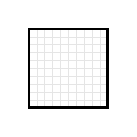
\begin{tikzpicture}[yscale=-1,
  mill/.style={line width=.1mm,gray!20},
  cent/.style={thick,gray!60}]
	\begin{scope}
		\clip (0,0) rectangle (\WW,\HH);
		\foreach \i in {1,...,180}
		\draw[mill] (\i*0.1,0) -- (\i*0.1,\HH);
		\foreach \i in {1,...,270}
		\draw[mill] (0,\i*0.1) -- (\WW,\i*0.1);
		\foreach \i in {1,...,18}
		\draw[cent] (\i,0) -- (\i,\HH);
		\foreach \i in {1,...,27}
		\draw[cent] (0,\i) -- (\WW,\i);
	\end{scope}
	\draw[line width=1pt] (0,0) rectangle (\WW,\HH);
\end{tikzpicture}

\begin{tikzpicture}[yscale=-1]
	\foreach \i in {1,...,\EOFmonth}
  \draw[gray!40] (0,\i * \spacin) -- (\WW,\i * \spacin) 
  node[above, pos=.05,black] {\i};
	\draw[line width=1pt] (0,0) rectangle (\WW,\HH);
\end{tikzpicture}

\def\EOFmonth{30}
\setlength{\spacin}{\HH / \EOFmonth}
\begin{tikzpicture}[yscale=-1]
	\foreach \i in {1,...,\EOFmonth}
  \draw[gray!40] (0,\i * \spacin) -- (\WW,\i * \spacin) 
  node[above, pos=.05,black] {\i};
	\draw[line width=1pt] (0,0) rectangle (\WW,\HH);
\end{tikzpicture}

\def\EOFmonth{28}
\setlength{\spacin}{\HH / \EOFmonth}
\begin{tikzpicture}[yscale=-1]
	\foreach \i in {1,...,\EOFmonth}
  \draw[gray!40] (0,\i * \spacin) -- (\WW,\i * \spacin) 
  node[above, pos=.05,black] {\i};
	\draw[line width=1pt] (0,0) rectangle (\WW,\HH);
\end{tikzpicture}

\begin{tikzpicture}[yscale=-1]
  \draw[line width=1pt] (0,0) rectangle (\WW,\HH);
  \draw (\WWh,0) -- (\WWh,\HH);
  \node[below right=.5cm] at (\WWh,0) {\sunday};
  \foreach \i/\j/\k in { 1/\monday/\tuesday
                       , 2/\wednesday/\thursday
                       , 3/\friday/\saturday
                       }
  \draw (0,\i * \HH/4) -- (\WW,\i * \HH/4) 
    node[pos=.5,below left =.5cm] {\large\j}
    node[pos=.5,below right=.5cm] {\large\k};
\end{tikzpicture}

\begin{tikzpicture}[yscale=-1]
  \draw[line width=1pt] (0,0) rectangle (.75\WW,\HH/2);
  \draw (.75\WWh,0) -- (.75\WWh,\HH/2);
  \node[below right=.5cm] at (.75\WWh,0) {\sunday};
  \foreach \i/\j/\k in { 1/\monday/\tuesday
                       , 2/\wednesday/\thursday
                       , 3/\friday/\saturday
                       }
  \draw (0,\i * \HH/8) -- (.75\WW,\i * \HH/8) 
    node[pos=.5,below left=.5cm] {\large\j}
    node[pos=.5,below right=.5cm] {\large\k};
    \begin{scope}[yshift=3/2 * \HHh + .75cm]
      \draw[line width=1pt] (0,0) rectangle (.75\WW,\HH/2);
      \draw (.75\WWh,0) -- (.75\WWh,\HH/2);
      \node[below right=.5cm] at (.75\WWh,0) {\sunday};
      \foreach \i/\j/\k in { 1/\monday/\tuesday
                           , 2/\wednesday/\thursday
                           , 3/\friday/\saturday
                           }
      \draw (0,\i * \HH/8) -- (.75\WW,\i * \HH/8) 
        node[pos=.5,below left=.5cm] {\large\j}
        node[pos=.5,below right=.5cm] {\large\k};
    \end{scope}
\end{tikzpicture}

\begin{tikzpicture}[yscale=-1]
  \fill[gray!15] (0,0) rectangle (\WW/4,.75\HH);
  \draw[line width=1pt] (\WW,0) -- (0,0) |- (\WW,0.75\HH);
  \foreach \i in {1,...,4}
  \draw[gray!40,ultra thin] (0,\i * 0.75\HH / 5) -- (\WW,\i * 0.75\HH / 5);
  \foreach \j/\k in {1/\sunday,2/\monday,3/\tuesday}{
  \draw (\j * \WW/4,0) -- (\j * \WW/4,0.75\HH);
  \draw[gray!40,yshift=4\HH/5] (0,0) rectangle (\WW,\HH/5);
  \node[gray!5, below right=.25cm] at (\j * \WW/4,0) {\k};
  }
\end{tikzpicture}

\begin{tikzpicture}[yscale=-1]
  \draw[line width=1pt] (0,0) -| (\WW,0.75\HH) -- (0,0.75\HH);
  \foreach \i in {1,...,4}
  \draw[gray!40,ultra thin] (0,\i * 0.75\HH / 5) -- (\WW,\i * 0.75\HH / 5);
  \foreach \j in {1,2,3}
  \draw (\j * \WW/4,0) -- (\j * \WW/4,0.75\HH);
  \draw[gray!40,yshift=4\HH/5] (0,0) rectangle (\WW,\HH/5);
  \foreach \j/\k in {0/\wednesday,1/\thursday,2/\friday,3/\saturday}
  \node[gray!5, below right=.25cm] at (\j * \WW/4,0) {\k};
\end{tikzpicture}
\end{document}
